\documentclass%
%[handout]
{beamer}
% % % % % % % %
% % % % % % % %
% % % % % % % %
%IMPORTANT
%compiles with 
%pdflatex -shell-escape 
%IMPORTANT
% % % % % % % %
% % % % % % % %
% % % % % % % %
\mode<presentation>
{
\useinnertheme{rounded}
\useoutertheme{infolines}
\usecolortheme{orchid}
\usecolortheme{whale}
}

\usepackage[english]{babel}
\usepackage[latin1]{inputenc}
\usepackage[all,cmtip]{xy}
\usepackage{times}
\usepackage[T1]{fontenc}
\usepackage{../example-templates}
\usepackage{../pstricks-commands}
\usepackage{cancel}

\usepackage{auto-pst-pdf}
\usepackage{pst-plot}
%\usepackage{pstricks-add} 

% Or whatever. Note that the encoding and the font should match. If T1
% does not look nice, try deleting the line with the fontenc.

\graphicspath{{../../modules/}}

\newtheoremstyle{partialproof}{3pt}{3pt}{}{}{}{.}{.5em}{}
\theoremstyle{partialproof} \newtheorem{partialproof}[theorem]{Proof.}
%\DeclareMathOperator{\diff}{d}
\newcommand{\diff}{\text{d}}
\setbeamertemplate{navigation symbols}{}

\includeonlylecture{1}

\newcommand{\lect}[3]{
  \date{#1}
  \lecture[#1]{#2}{#3}
}

\setbeamertemplate{footline}
{
  \leavevmode%
  \hbox{%
  \begin{beamercolorbox}[wd=.333333\paperwidth,ht=2.25ex,dp=1ex,center]{author in head/foot}%
    \usebeamerfont{author in head/foot}\insertshortauthor
  \end{beamercolorbox}%
  \begin{beamercolorbox}[wd=.333333\paperwidth,ht=2.25ex,dp=1ex,center]{title in head/foot}%
    \usebeamerfont{title in head/foot}\insertshorttitle
  \end{beamercolorbox}%
  \begin{beamercolorbox}[wd=.333333\paperwidth,ht=2.25ex,dp=1ex,center]{date in head/foot}%
    \usebeamerfont{date in head/foot}\insertshortdate{}
  \end{beamercolorbox}}%
  \vskip0pt%
}

% If you have a file called "university-logo-filename.xxx", where xxx
% is a graphic format that can be processed by latex or pdflatex,
% resp., then you can add a logo as follows:

%\pgfdeclareimage[height=0.8cm]{logo}{bluelogo}
%\logo{\pgfuseimage{logo}}

\begin{document}

\AtBeginLecture{%

\title[\insertlecture]{FreeCalc}
\subtitle{\insertlecture}
\author[FreeCalc]{}
\institute[UMass Boston]{University of Massachusetts Boston}
\date{\insertshortlecture}
\begin{frame}
  \titlepage
\end{frame}
}%

% begin lecture
\lect{\today}{Sample}{1}
%% begin module FTC-intro
\begin{frame}
\frametitle{(5.3) The Fundamental Theorem of Calculus}
\begin{itemize}
\item  The Fundamental Theorem of Calculus establishes a connection between differential calculus and integral calculus.
\item  It allows us to compute integrals very easily, without finding limits of Riemann sums.
\item  It has two different parts.
\item  Part 1 says, roughly, that ``differentiation undoes integration.''
\item  Part 2 says, roughly, that ``integration undoes differentiation.''
\item<2->  Part 1 deals with functions of the form
\[
\uncover<2->{%
g(x) = \int_a^x  f(t) \diff t%
}%
\]
\uncover<2->{where $f$ is a continuous function on $[a,b]$ and $x$ varies between $a$ and $b$.}
\end{itemize}
\end{frame}
% end module FTC-intro

%% begin module definite-integral-properties-split
\begin{frame}[t]
Properties of the Integral
\begin{enumerate}
\setcounter{enumi}{4}
\item  $\displaystyle %
\alertNoH{ 1}{\int_a^b f(x) \diff x} %
= %
\alertNoH{ 2}{\int_a^c f(x) \diff x} %
+ %
\alertNoH{ 3}{\int_c^b f(x) \diff x} %
$%
\end{enumerate}
\begin{center}
\psset{xunit=1.5cm, yunit=1.5cm}
\begin{pspicture}(-0.5,-0.5)(4.5,3.6)
\psframe*[linecolor=white](-0.5,-0.5)(4.5,3.6)
%Function formula: 1727/6250+4911/100 ((x)^{3})+110043/5000 (x)+3 ((x)^{5})-201/10 ((x)^{4})-52431/1000 ((x)^{2})
\uncover<1>{
\pscustom*[linecolor=\fcColorAreaUnderGraph]{
\psplot[linecolor=red, plotpoints=1000]{0.1}{2.5}{x 2 exp -52.431 mul x 4 exp -20.1 mul x 5 exp 3 mul x 22.0086 mul x 3 exp 49.11 mul 0.27632 add add add add add }
\psline(2.5, 0)(0.1,0)
}
}
\uncover<2>{
\pscustom*[linecolor=\fcColorAreaUnderGraph]{
\psplot[linecolor=red, plotpoints=1000]{0.1}{1.7}{x 2 exp -52.431 mul x 4 exp -20.1 mul x 5 exp 3 mul x 22.0086 mul x 3 exp 49.11 mul 0.27632 add add add add add }
\psline(1.7, 0)(0.1,0)
}
}
\uncover<3>{
\pscustom*[linecolor=\fcColorAreaUnderGraph]{
\psplot[linecolor=red, plotpoints=1000]{1.7}{2.5}{x 2 exp -52.431 mul x 4 exp -20.1 mul x 5 exp 3 mul x 22.0086 mul x 3 exp 49.11 mul 0.27632 add add add add add }
\psline(2.5, 0)(1.7,0)
}
}

\psline(0.1, 0.05)(0.1, -0.05)
\rput[t](0.1, -0.07){$a$}
\psline(1.7, 0.05)(1.7, -0.05)
\rput[t](1.7, -0.07){$c$}
\psline(2.5, 0.05)(2.5, -0.05)
\rput[t](2.5, -0.07){$b$}
\rput(1.5, 2.4 ){$y=f(x)$}
\psaxes[ticks=none, labels=none]{<->}(0,0)(-0.5,-0.5)(4,2.7)\tiny
\psplot[linecolor=red, plotpoints=1000]{0.1}{2.5}{x 2 exp -52.431 mul x 4 exp -20.1 mul x 5 exp 3 mul x 22.0086 mul x 3 exp 49.11 mul 0.27632 add add add add add }
\end{pspicture}
%\only<handout:0| -1>{%
%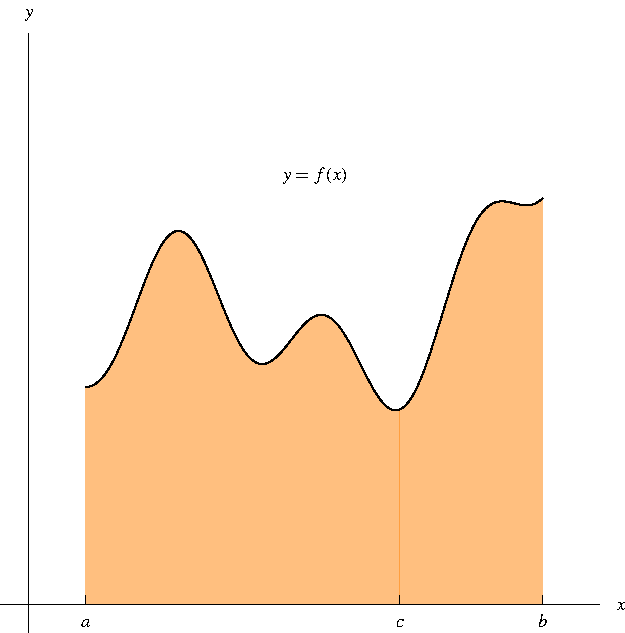
\includegraphics[height=5.6cm]{integration/pictures/05-02-splita.pdf}%
%}%
%\only<handout:0| 2>{%
%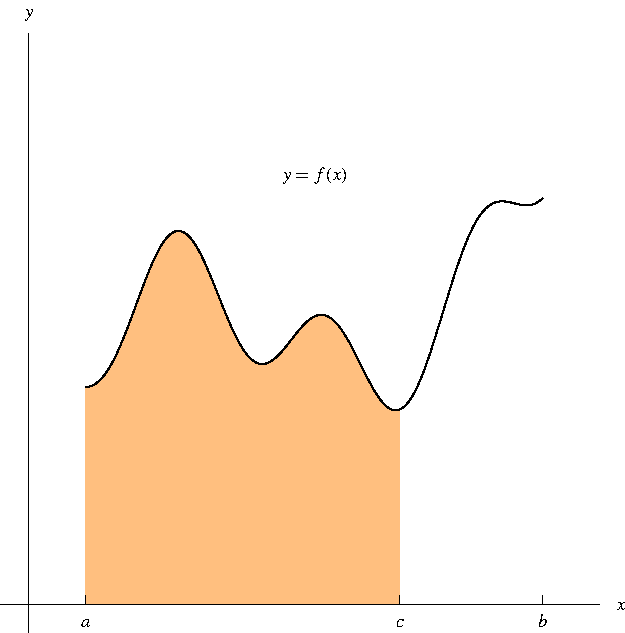
\includegraphics[height=5.6cm]{integration/pictures/05-02-splitb.pdf}%
%}%
%\only<handout:0| 3>{%
%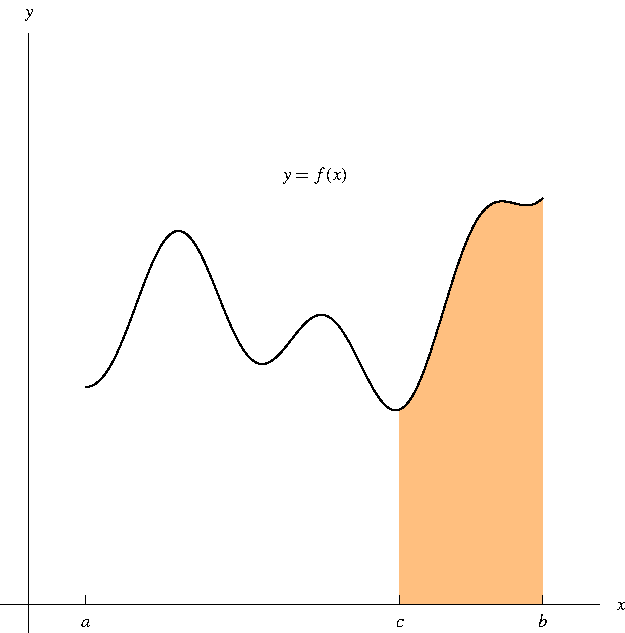
\includegraphics[height=5.6cm]{integration/pictures/05-02-splitc.pdf}%
%}%
\end{center}
\end{frame}
% end module definite-integral-properties-split

%% begin module definite-integral-properties-ex7
\begin{frame}
\begin{example} %[Example 7, p. 352]
If it is known that \alert<handout:0| 5-6>{$\int_0^{10}f(x)\diff x = 17$} and \alert<handout:0| 7-8>{$\int_0^8 f(x) \diff x = 12$}, then find $\int_8^{10}f(x) \diff x$.
\abovedisplayskip=0pt
\belowdisplayskip=0pt
\abovedisplayshortskip=0pt
\belowdisplayshortskip=0pt
\begin{align*}
\uncover<2->{%
\int_{\alert<handout:0| 2-3>{0}}^{\alert<handout:0| 2-3>{8}} f(x)\diff x + \int_{\alert<handout:0| 2-3>{8}}^{\alert<handout:0| 2-3>{10}}f(x)\diff x%
}%
& \uncover<3->{ = } %
\uncover<3->{%
\int_{\alert<handout:0| 3>{0}}^{\alert<handout:0| 3>{10}}f(x)\diff x%
}\\%
\uncover<4->{%
\int_{\alert<handout:0| 2-3>{8}}^{\alert<handout:0| 2-3>{10}}f(x)\diff x%
}%
& \uncover<4->{ = } %
\uncover<4->{%
\alert<handout:0| 5-6>{\int_{\alert<handout:0| 3>{0}}^{\alert<handout:0| 3>{10}}f(x)\diff x} - \alert<handout:0| 7-8>{\int_{\alert<handout:0| 2-3>{0}}^{\alert<handout:0| 2-3>{8}} f(x)\diff x}%
}\\%
& \uncover<5->{ = } %
\uncover<5->{%
\alert<handout:0| 5-6>{\uncover<6->{17}} - \alert<handout:0| 7-8>{\uncover<8->{12}}%
}\\%
& \uncover<9->{ = } %
\uncover<9->{%
5%
}%
\end{align*}
\end{example}
\end{frame}
% end module definite-integral-properties-ex7

% WARNING: This next module could use some pictures.
%% begin module definite-integral-properties-comparison
\begin{frame}[t]
Comparison Properties of the Integral
\begin{enumerate}
\setcounter{enumi}{5}
\item  If $f(x)\geq 0$ for all $a\leq x \leq b$, then $\displaystyle \int_{a}^{b} f(x)\diff x \geq 0$.
\end{enumerate}
\end{frame}

\begin{frame}[t]
Comparison Properties of the Integral
\begin{enumerate}
\setcounter{enumi}{6}
\item  If $f(x)\leq g(x)$ for all $a\leq x \leq b$, then $\displaystyle \int_{a}^{b} f(x)\diff x \leq \int_{a}^{b} g(x)\diff x$.
\end{enumerate}
\begin{center}
\psset{xunit=0.9cm, yunit=0.9cm}
\begin{pspicture}(-0.5,-0.5)(6,4.5)
\psframe*[linecolor=white](-0.5,-0.5)(6,4.5)
\tiny
\rput[l](5.1, 2.6){$y=g(x)$}
\rput[l](5.1, 1.3){$y=f(x)$}
\uncover<2>{
\pscustom*[linecolor=cyan]{
\psplot[linecolor=red, plotpoints=1000]{0.2}{5}{x 2 exp -0.18 mul x 3 exp 0.025 mul x 0.368 mul 0.808 add add add }
\psline(5,0)(0.2,0)
}
}
\uncover<3->{
\pscustom*[linecolor=cyan]{
\psplot[linecolor=red, plotpoints=1000]{0.2}{5}{x -9.9495 mul x 3 exp -2.0625 mul x 4 exp 0.1875 mul x 2 exp 7.4925 mul 5.6936 add add add add }
\psline(5,0)(0.2,0)
}
}
%Function formula: 101/125+46/125 (x)+1/40 ((x)^{3})-9/50 ((x)^{2})
\psplot[linecolor=red, plotpoints=1000]{0.2}{5}{x 2 exp -0.18 mul x 3 exp 0.025 mul x 0.368 mul 0.808 add add add }
%Function formula: 7117/1250+2997/400 ((x)^{2})+3/16 ((x)^{4})-33/16 ((x)^{3})-19899/2000 (x)
\psaxes[ticks=none, labels=none]{<->}(0,0)(-0.5,-0.5)(6,4.5)
\psplot[linecolor=red, plotpoints=1000]{0.2}{5}{x -9.9495 mul x 3 exp -2.0625 mul x 4 exp 0.1875 mul x 2 exp 7.4925 mul 5.6936 add add add add }
\psline(0.2, -0.1)(0.2, 0.1)
\rput[t](0.2, -0.15){$a$}
\psline(5, -0.1)(5, 0.1)
\rput[t](5, -0.15){$b$}
\end{pspicture}
%\only<handout:0| -1>{%
%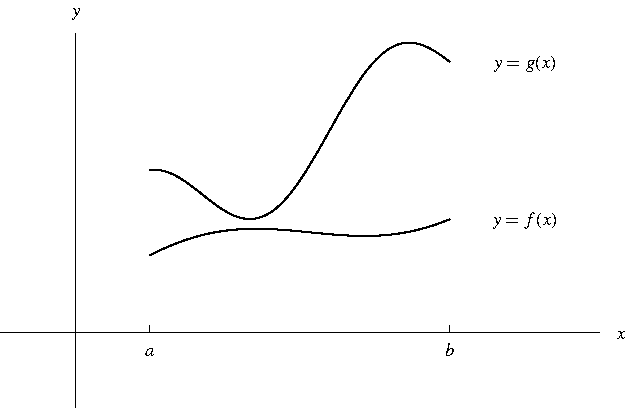
\includegraphics[height=4.2cm]{integration/pictures/05-02-comparisona.pdf}%
%}%
%\only<handout:0| 2>{%
%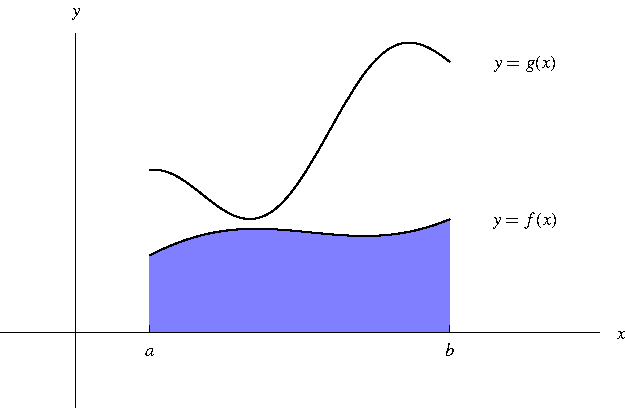
\includegraphics[height=4.2cm]{integration/pictures/05-02-comparisonb.pdf}%
%}%
%\only<handout:0| 3>{%
%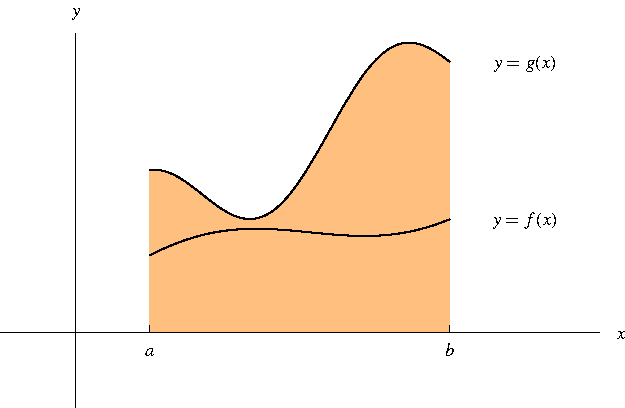
\includegraphics[height=4.2cm]{integration/pictures/05-02-comparisonc.pdf}%
%}%
\[
\alertNoH{ 2}{\int_a^b f(x) \diff x}%
 \leq  %
\alertNoH{ 3}{\int_a^b g(x) \diff x}%
\]
\end{center}
\end{frame}

\begin{frame}[t]
Comparison Properties of the Integral
\begin{enumerate}
\setcounter{enumi}{7}
\item  If $m\leq f(x)\leq M$ for all $a\leq x \leq b$, then
\[
\alertNoH{ 2}{m(b-a)}%
 \leq  %
\alertNoH{ 3}{\int_a^b f(x) \diff x}%
 \leq  %
\alertNoH{ 4}{M(b-a)}%
\]
\end{enumerate}
\begin{center}
\psset{xunit=0.9cm, yunit=0.9cm}
\begin{pspicture}(-0.5,-0.5)(6,4.5)
\psframe*[linecolor=white](-0.5,-0.5)(6,4.5)
\tiny
\uncover<2>{
\pscustom*[linecolor=orange]{
\psplot[linecolor=\fcColorGraph, plotpoints=1000]{0.2}{5}{0.7}
\psline(5,0)(0.2,0)
}
}

\uncover<3>{
\pscustom*[linecolor=cyan!50]{
\psplot[linecolor=\fcColorGraph, plotpoints=1000]{0.2}{5}{x -9.9495 mul x 3 exp -2.0625 mul x 4 exp 0.1875 mul x 2 exp 7.4925 mul 5.6936 add add add add }
\psline(5,0)(0.2,0)
}
}
\uncover<4>{
\pscustom*[linecolor=cyan]{
\psplot[linecolor=red, plotpoints=1000]{0.2}{5}{4.3}
\psline(5,0)(0.2,0)
}
}
%Function formula: 7117/1250+2997/400 ((x)^{2})+3/16 ((x)^{4})-33/16 ((x)^{3})-19899/2000 (x)
\psaxes[ticks=none, labels=none]{<->}(0,0)(-0.5,-0.5)(6,4.5)
\psplot[linecolor=\fcColorGraph, plotpoints=1000]{0.2}{5}{x -9.9495 mul x 3 exp -2.0625 mul x 4 exp 0.1875 mul x 2 exp 7.4925 mul 5.6936 add add add add }
\psline[linecolor=\fcColorGraph](0.2, 0.7)(5,0.7)
\psline[linecolor=\fcColorGraph](0.2, 4.3)(5, 4.3)


\rput[r](4.9, 2.6){\alertNoH{3}{$y=f(x)$}}
\psline[linestyle=dotted, arrows=<->](5.05, 0)(5.05, 0.7)
\rput[l](5.15,0.35){\alertNoH{2}{$m$}}
\psline[linestyle=dotted, arrows=<->](5.5, 0)(5.5, 4.3)
\rput[l](5.6,2.15){\alertNoH{4}{$M$}}

\psline(0.2, -0.1)(0.2, 0.1)
\rput[t](0.2, -0.15){\alertNoH{2,4}{$a$}}
\psline(5, -0.1)(5, 0.1)
\rput[t](5, -0.15){\alertNoH{2,4}{$b$}}
\end{pspicture}
%\only<handout:0| -1>{%
%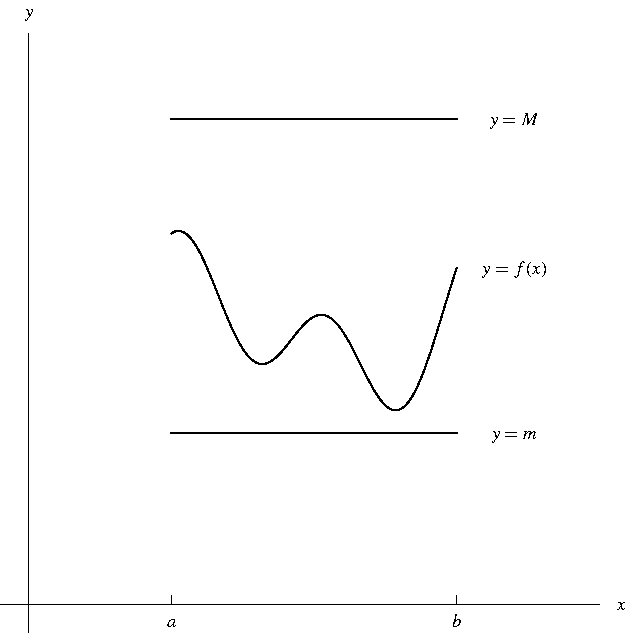
\includegraphics[height=5.6cm]{integration/pictures/05-02-boundinga.pdf}%
%}%
%\only<handout:0| 2>{%
%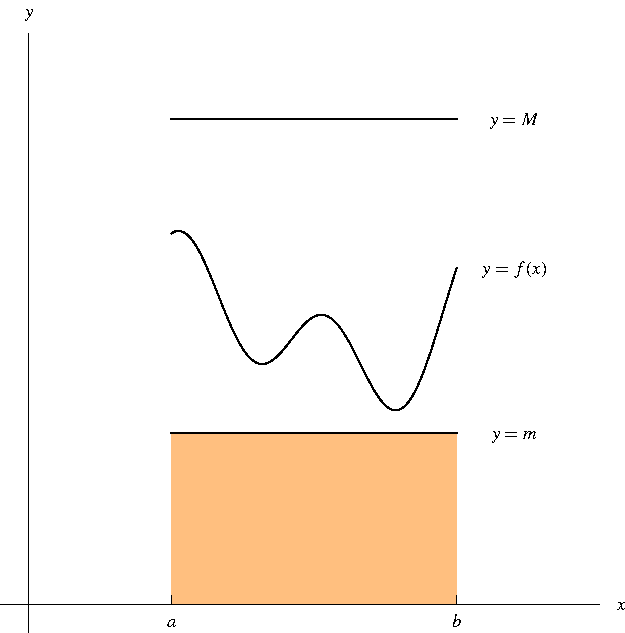
\includegraphics[height=5.6cm]{integration/pictures/05-02-boundingb.pdf}%
%}%
%\only<handout:0| 3>{%
%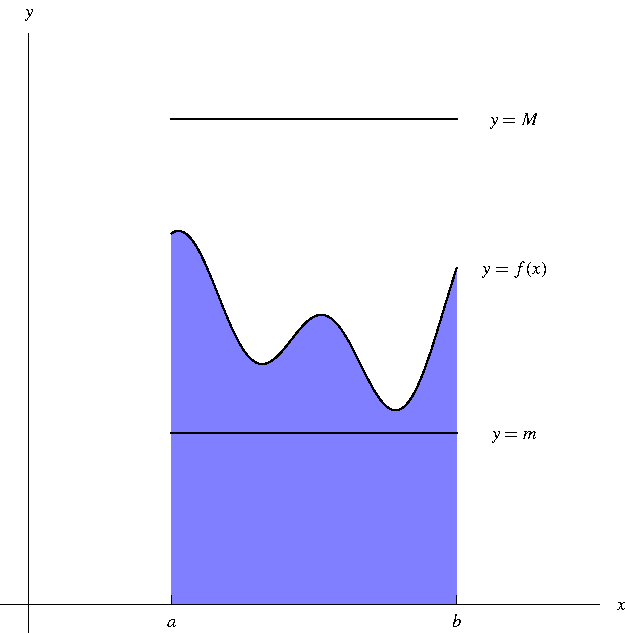
\includegraphics[height=5.6cm]{integration/pictures/05-02-boundingc.pdf}%
%}%
%\only<handout:0| 4>{%
%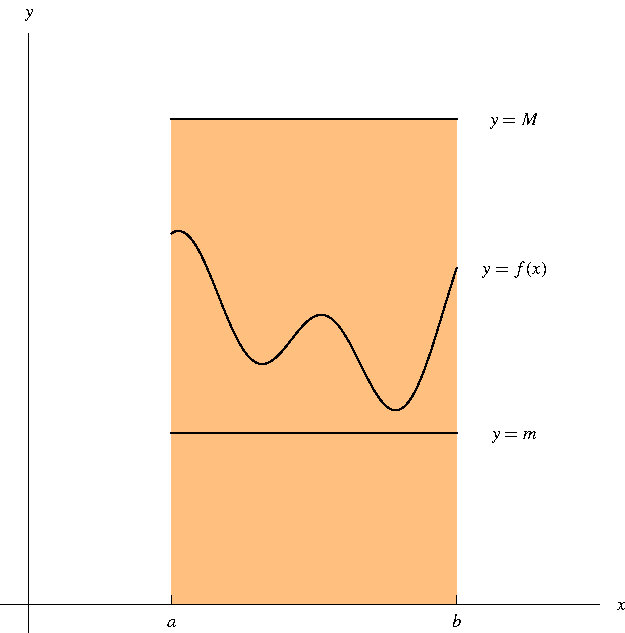
\includegraphics[height=5.6cm]{integration/pictures/05-02-boundingd.pdf}%
%}%
\end{center}
\end{frame}
% end module definite-integral-properties-comparison

%% begin module FTC-part2-ex7
\begin{frame}
\begin{example} %[Example 2, p. 357]
\begin{columns}
\column{0.2\textwidth}
\psset{xunit=0.4cm, yunit=0.4cm}
\begin{pspicture}(-1.000000, -5)(1.500000,5) 
\psframe*[linecolor=white](-1.000000,-5)(7,5) 
\tiny 
\pscustom*[linecolor=cyan]{ %Function formula: \cos{}x 
\psplot[linecolor=\psColorGraph, plotpoints=1000]{0}{1}{x 57.29578 mul cos }\psline(1.000000, 0)(0.000000, 0)}
%Function formula: \cos{}x 
\psplot[linecolor=\psColorGraph, plotpoints=1000]{0}{6}{x 57.29578 mul cos }
\psaxesStandard{-0.6}{-0.6}{6}{1.1}
\end{pspicture} 
\column{0.8\textwidth}
Find the area under the cosine curve from $0$ to $b$, where $0 \leq b \leq \pi /2$.
\begin{itemize}
\item<2->  $\cos x$ is continuous on $[0, \pi /2]$ (in fact, it's continuous everywhere).
\item<3-| alert@3-4>  An antiderivative is \uncover<4->{$\sin x$.}
\end{itemize}
\[
\uncover<5->{%
\int_{\alert<handout:0| 5>{0}}^{\alert<handout:0| 5>{b}} \cos x \ \diff x = \left[ \sin x \right]_{\alert<handout:0| 5>{0}}^{\alert<handout:0| 5>{b}} %
}%
\uncover<6->{%
 = \sin (b) - \sin (0)%
}%
\uncover<7->{%
 = \sin b%
}%
\]
\end{columns}
\end{example}
\end{frame}
% end module FTC-part2-ex7

%% begin module area-def
\begin{frame}
Estimate the area under the curve $y = f(x)$ between $a$ and $b$.
\begin{columns}
\column{.55\textwidth}
\psset{xunit=3cm, yunit=3cm}
\begin{pspicture}(-5, -5)(5,5)
\psframe*[linecolor=white](-5,-5)(5,5)
\psaxes[ticks=none, labels=none]{<->}(0,0)(-0.1,-0.1)(1.7,0.9)
\tiny

\uncover<1>{
\psline*[linecolor=\fcColorAreaUnderGraph, linewidth=0.1pt](0.425, 0)(0.425, 0.339931)(0.3, 0.339931)(0.3, 0)(0.55, 0)(0.55, 0.316508)(0.425, 0.316508)(0.425, 0)(0.675, 0)(0.675, 0.348456)(0.55, 0.348456)(0.55, 0)(0.8, 0)(0.8, 0.416)(0.675, 0.416)(0.675, 0)(0.925, 0)(0.925, 0.499364)(0.8, 0.499364)(0.8, 0)(1.05, 0)(1.05, 0.578773)(0.925, 0.578773)(0.925, 0)(1.175, 0)(1.175, 0.634452)(1.05, 0.634452)(1.05, 0)(1.3, 0)(1.3, 0.646625)(1.175, 0.646625)(1.175, 0)(1.425, 0)(1.425, 0.595517)(1.3, 0.595517)(1.3, 0)(1.55, 0)(1.55, 0.461352)(1.425, 0.461352)(1.425, 0)
\psline[linecolor=blue, linewidth=0.1pt](0.425, 0)(0.425, 0.339931)(0.3, 0.339931)(0.3, 0)(0.55, 0)(0.55, 0.316508)(0.425, 0.316508)(0.425, 0)(0.675, 0)(0.675, 0.348456)(0.55, 0.348456)(0.55, 0)(0.8, 0)(0.8, 0.416)(0.675, 0.416)(0.675, 0)(0.925, 0)(0.925, 0.499364)(0.8, 0.499364)(0.8, 0)(1.05, 0)(1.05, 0.578773)(0.925, 0.578773)(0.925, 0)(1.175, 0)(1.175, 0.634452)(1.05, 0.634452)(1.05, 0)(1.3, 0)(1.3, 0.646625)(1.175, 0.646625)(1.175, 0)(1.425, 0)(1.425, 0.595517)(1.3, 0.595517)(1.3, 0)(1.55, 0)(1.55, 0.461352)(1.425, 0.461352)(1.425, 0)
}
\uncover<2->{
\psline*[linecolor=\fcColorAreaUnderGraph, linewidth=0.1pt](0.3, 0)(0.3, 0.4385)(0.425, 0.4385)(0.425, 0)(0.425, 0)(0.425, 0.339931)(0.55, 0.339931)(0.55, 0)(0.55, 0)(0.55, 0.316508)(0.675, 0.316508)(0.675, 0)(0.675, 0)(0.675, 0.348456)(0.8, 0.348456)(0.8, 0)(0.8, 0)(0.8, 0.416)(0.925, 0.416)(0.925, 0)(0.925, 0)(0.925, 0.499364)(1.05, 0.499364)(1.05, 0)(1.05, 0)(1.05, 0.578773)(1.175, 0.578773)(1.175, 0)(1.175, 0)(1.175, 0.634452)(1.3, 0.634452)(1.3, 0)(1.3, 0)(1.3, 0.646625)(1.425, 0.646625)(1.425, 0)(1.425, 0)(1.425, 0.595517)(1.55, 0.595517)(1.55, 0)
\psline[linecolor=blue, linewidth=0.1pt](0.3, 0)(0.3, 0.4385)(0.425, 0.4385)(0.425, 0)(0.425, 0)(0.425, 0.339931)(0.55, 0.339931)(0.55, 0)(0.55, 0)(0.55, 0.316508)(0.675, 0.316508)(0.675, 0)(0.675, 0)(0.675, 0.348456)(0.8, 0.348456)(0.8, 0)(0.8, 0)(0.8, 0.416)(0.925, 0.416)(0.925, 0)(0.925, 0)(0.925, 0.499364)(1.05, 0.499364)(1.05, 0)(1.05, 0)(1.05, 0.578773)(1.175, 0.578773)(1.175, 0)(1.175, 0)(1.175, 0.634452)(1.3, 0.634452)(1.3, 0)(1.3, 0)(1.3, 0.646625)(1.425, 0.646625)(1.425, 0)(1.425, 0)(1.425, 0.595517)(1.55, 0.595517)(1.55, 0)
}
\rput[t](0.3,-0.03){$a$}
\rput[t](0.425,-0.03){$x_1$}
\rput[t](0.55,-0.03){$x_2$}
%\rput[t](0.675,-0.03){}
%\rput[t](0.8,-0.03){$\frac{4}{5}$}
\rput[t](0.7375,-0.06){$\dots$}
\rput[t](0.925,-0.03){$x_{i-1}$}
\rput[t](1.05,-0.03){$x_{i}$}
%\rput[t](1.175,-0.03){$x_i$}
%\rput[t](1.3,-0.03){$\frac{13}{10}$}
\rput[t](1.3,-0.06){$\dots$}
%\rput[t](1.425,-0.03){$\frac{57}{40}$}
\rput[t](1.55,-0.03){$b$}
%Function formula: -171/50 (x)-27/16 ((x)^{3})+11/10+729/160 ((x)^{2})
\psplot[linecolor=red, plotpoints=1000]{0.3}{1.55}{x 2 exp 4.55625 mul 1.1 add x 3 exp -1.6875 mul add x -3.42 mul add }
\psline{<->}(1.6,0)(1.6, 0.578773)
\psline[linestyle=dotted](1.6, 0.578773)(1.05, 0.578773)
\rput[l](1.6, 0.3343865){$f(x_i)$}
\rput[b](0.9875,0.70773){$\Delta x$}
\psline(0.925,0.668773)(1.05, 0.668773)
\psline(0.925,0.648773)(0.925,0.688773)
\psline(1.05, 0.648773)(1.05, 0.688773)

%\psbrace[linecolor=red,ref=lC](2)(3){Text I}
%\uput{:U}{$\overbrace{}^\text{\normalsize A line}$}
\end{pspicture}
%\only<handout:1| -1>{%
%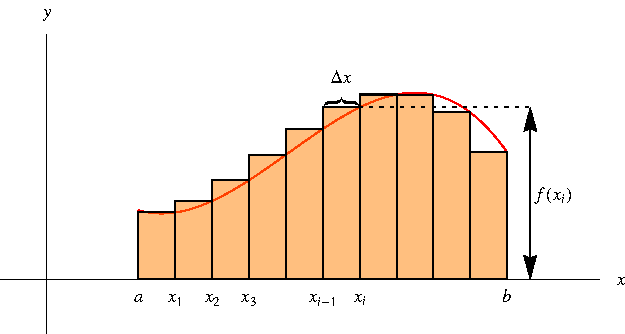
\includegraphics[height=3.5cm]{integration/pictures/05-01-rectangles-right.pdf}%
%}%
%\only<handout:2| 2->{%
%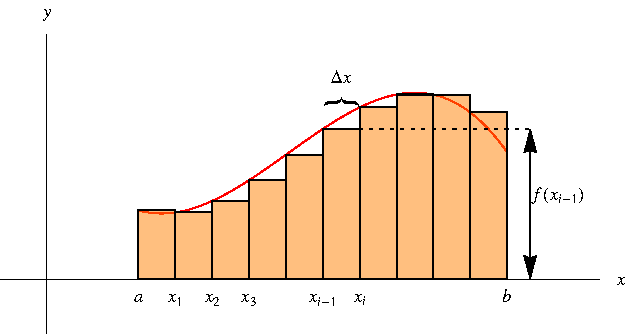
\includegraphics[height=3.5cm]{integration/pictures/05-01-rectangles-left.pdf}%
%}%



\begin{itemize}
\item<1->  The width of the interval is $b-a$.
\item<1->  The width of each of the $n$ strips is $\Delta x = \frac{b-a}{n}$.
\item<1->  The strips divide $[a,b]$ into $n$ subintervals:\\ $[x_0, x_1]$, $[x_1,x_2]$, $\ldots ,$ $[x_{n-1},x_n]$,\\ where $x_0 = a$ and $x_n = b$.
\end{itemize}
\column{.45\textwidth}
\begin{itemize}
\item<1->  The \only<handout:1| -1>{right}\only<handout:2| 2->{\alert<handout:2| 2>{left}} endpoints of the subintervals are
\end{itemize}
\abovedisplayskip=0pt
\belowdisplayskip=0pt
\begin{eqnarray*}
x_{\only<handout:1| -1>{1}\only<handout:2| 2->{\alert<handout:2| 2>{0}}} & = & a \only<handout:1| -1>{+ \Delta x}\\
x_{\only<handout:1| -1>{2}\only<handout:2| 2->{\alert<handout:2| 2>{1}}} & = & a + \only<handout:1| -1>{2}\Delta x\\
x_{\only<handout:1| -1>{3}\only<handout:2| 2->{\alert<handout:2| 2>{2}}} & = & a + \only<handout:1| -1>{3}\only<handout:2| 2->{2}\Delta x\\
& \vdots &
\end{eqnarray*}
\begin{itemize}
\item<1->  The height of the $i$th rectangle is $f(x_{i\only<handout:2| 2->{\alert<handout:2| 2>{-1}}})$.
\item<1->  The area of the $i$th rectangle is $f(x_{i\only<handout:2| 2->{\alert<handout:2| 2>{-1}}})\Delta x$.
\end{itemize}
\end{columns}
\abovedisplayskip=0pt
\belowdisplayskip=0pt
\[
\only<handout:1| -1>{R_n}\only<handout:2| 2->{\alert<handout:2| 2>{L_n}} = f(x_{\only<handout:1| -1>{1}\only<handout:2| 2->{\alert<handout:2| 2>{0}}})\Delta x + f(x_{\only<handout:1| -1>{2}\only<handout:2| 2->{\alert<handout:2| 2>{1}}})\Delta x + f(x_{\only<handout:1| -1>{3}\only<handout:2| 2->{\alert<handout:2| 2>{2}}})\Delta x + \cdots + f(x_{n\only<handout:2| 2->{\alert<handout:2| 2>{-1}}})\Delta x
\]
\end{frame}

\begin{frame}
\begin{definition}[Area Under a Curve]
The area of the region $S$ that lies under the curve $y = f(x)$ is the limit of the sum of the areas of the approximating rectangles:
\abovedisplayskip=0pt
\belowdisplayskip=0pt
\[
A = \lim_{n\to\infty} R_n = \lim_{n\to\infty} [ f(x_1)\Delta x + f(x_2) \Delta x + \cdots + f(x_n) \Delta x]
\]
\end{definition}
\begin{itemize}
\item<2->  This limit always exists if $f$ is continuous.
\item<3->  If $f$ is continuous, we get the same limit if we use left endpoints:
\abovedisplayskip=0pt
\belowdisplayskip=0pt
\[
A = \lim_{n\to\infty} L_n = \lim_{n\to\infty} [ f(x_0)\Delta x + f(x_1) \Delta x + \cdots + f(x_{n-1}) \Delta x]
\]
\item<4->  If $f$ is continuous, we get the same limit if we use any number $x_i^*$ in the interval $[x_{i-1},x_i]$.  $x_i^*$ is called a sample point.
\abovedisplayskip=0pt
\belowdisplayskip=0pt
\[
A = \lim_{n\to\infty} [ f(x_1^*)\Delta x + f(x_2^*) \Delta x + \cdots + f(x_{n}^*) \Delta x]
\]
\end{itemize}
\uncover<5->{%
\begin{definition}[Riemann Sum]
A Riemann sum is any sum of the form
\abovedisplayskip=0pt
\belowdisplayskip=0pt
\[
f(x_1^*)\Delta x + f(x_2^*) \Delta x + \cdots + f(x_{n}^*) \Delta x.
\]
\end{definition}
}%
\end{frame}
% end module area-def

%% begin module definite-integral-def
\begin{frame}\frametitle{ %(5.2) 
The Definite Integral}
\begin{definition}[Definite Integral]
\begin{itemize}
\item  Let $f$ be a function defined for $a\leq x\leq b$.
\item  Divide the interval $[a,b]$ into $n$ subintervals of equal width $\Delta x = (b-a)/n$ nd set $x_0=a$, $x_n=b$.
\item  Let $x_0$, $x_1,\ldots ,$ $x_n $ be the endpoints of the subintervals.
\item  Let $x_1^*, x_2^*, \ldots , x_n^*$ be any sample points in these subintervals; that is, $x_i^*$ is in $[x_{i-1},x_i]$.  
\end{itemize}
\abovedisplayskip=0pt
\belowdisplayskip=0pt
Suppose the limit $\lim\limits_{n\to \infty} \sum\limits_{i=1}^n f(x_i^*)\Delta x$ exists and is independent of the choice of sample points $x_i^*$. Then we call this limit the integral of $f$ over $[a,b]$ and write
\[
\int_a^b f(x) \diff x = \lim_{n\to \infty} \sum_{i=1}^n f(x_i^*)\Delta x \quad .
\]
\end{definition}
\end{frame}

\begin{frame}
\[
\mathop{\alert<handout:0| 2>{\int}}_{\alert<handout:0| 4>{a}}^{\alert<handout:0| 4>{b}} \alert<handout:0| 3>{f(x)} \alert<handout:0| 0>{\diff x} = \lim_{n\to \infty} \sum_{i=1}^n f(x_i^*)\Delta x,
\]
\begin{itemize}
\item<1-| alert@2>  $\int$ is called the integration sign.
\item<1-| alert@3>  $f(x)$ is called the integrand.
\item<1-| alert@4>  $a$ and $b$ are called the limits of integration.
\item<5->  The definite integral is a number.  It does not depend on $x$.  We could use any variable instead of $x$.
\end{itemize}
\uncover<5->{%
\[
\int_a^b f(x) \diff x = \int_a^b f(t)\diff t = \int_a^b f(r)\diff r = \int_a^b f(\theta )\diff \theta
\]
}%
\end{frame}
% end module definite-integral-def

%% begin module FTC-part2
\begin{frame}
\uncover<3->{
\begin{theorem}
Let $f$ be a continuous function on $[a,b]$. Then $f$ is integrable over $[a,b]$.
\end{theorem}
}
\uncover<2->{
\uncover<3->{In other words,} \alert<2>{$\displaystyle\int_a^{b}f(x)dx $ is defined for any continuous (over $[a,b]$) function $f$}.
}

\begin{theorem}[The Evaluation Theorem (FTC part 2)]
If \alert<2>{$f$ is continuous on $[a, b]$}, then
\[
\alert<2>{\int_a^b f(x) \diff x} = F(b) - F(a),
\]
where $F$ is any antiderivative of $f$.
\end{theorem}

\end{frame}
% end module FTC-part2


%% begin module definite-integral-def
\begin{frame}\frametitle{ %(5.2) 
The Definite Integral}
\begin{definition}[Definite Integral]
\begin{itemize}
\item  Let $f$ be a function defined for $a\leq x\leq b$.
\item  Divide the interval $[a,b]$ into $n$ subintervals of equal width $\Delta x = (b-a)/n$ nd set $x_0=a$, $x_n=b$.
\item  Let $x_0$, $x_1,\ldots ,$ $x_n $ be the endpoints of the subintervals.
\item  Let $x_1^*, x_2^*, \ldots , x_n^*$ be any sample points in these subintervals; that is, $x_i^*$ is in $[x_{i-1},x_i]$.  
\end{itemize}
\abovedisplayskip=0pt
\belowdisplayskip=0pt
Suppose the limit $\lim\limits_{n\to \infty} \sum\limits_{i=1}^n f(x_i^*)\Delta x$ exists and is independent of the choice of sample points $x_i^*$. Then we call this limit the integral of $f$ over $[a,b]$ and write
\[
\int_a^b f(x) \diff x = \lim_{n\to \infty} \sum_{i=1}^n f(x_i^*)\Delta x \quad .
\]
\end{definition}
\end{frame}

\begin{frame}
\[
\mathop{\alert<handout:0| 2>{\int}}_{\alert<handout:0| 4>{a}}^{\alert<handout:0| 4>{b}} \alert<handout:0| 3>{f(x)} \alert<handout:0| 0>{\diff x} = \lim_{n\to \infty} \sum_{i=1}^n f(x_i^*)\Delta x,
\]
\begin{itemize}
\item<1-| alert@2>  $\int$ is called the integration sign.
\item<1-| alert@3>  $f(x)$ is called the integrand.
\item<1-| alert@4>  $a$ and $b$ are called the limits of integration.
\item<5->  The definite integral is a number.  It does not depend on $x$.  We could use any variable instead of $x$.
\end{itemize}
\uncover<5->{%
\[
\int_a^b f(x) \diff x = \int_a^b f(t)\diff t = \int_a^b f(r)\diff r = \int_a^b f(\theta )\diff \theta
\]
}%
\end{frame}
% end module definite-integral-def

%% begin module continuous-functions-integrable
\begin{frame}
\begin{theorem}
Let $f$ be a continuous function on $[a,b]$. Then $f$ is integrable over $[a,b]$.
\end{theorem}
\begin{itemize}
\item In particular the integral does not depend the choice of sampling points so long as the intervals containing them shrink.
\item The proof of this theorem is not difficult, but is outside of the scope of Calculus I and II.
\item The only ``difficulty'' in the proof stems from the fact that we have not rigorously constructed the real numbers. 
\item We already (silently) assumed a construction of the real numbers when we defined limits. 
\item Such a construction is also (silently) assumed in most regular high school mathematics courses.
%\item  The proof of the Theorem uses the fact that every set bounded above has a least upper bound. The latter fact is either taken as an axiom of the real numbers, or is proven from equivalent set of axioms. This is the main fact a calculus student is missing to understand/prove on one's own the above theorem.
\item A student interested in a proof of the theorem should google ``Darboux integral''.
\end{itemize}

\end{frame}
% end module continuous-functions-integrable

% begin module FTC1-proof
\begin{frame}
\begin{theorem}[The Fundamental Theorem of Calculus part 1]
Let \alertNoH{2}{$f$ be a function continuous on $[a, b]$} and let $G(x) = \displaystyle \int_a^x f(t) \diff t$ for all $x\in [a,b]$. Then $G$ is differentiable and $G'(x) = f(x)$.
\end{theorem}
\begin{proof}[Proof]
\begin{columns}
\column{0.27\textwidth}
\psset{xunit=0.9cm, yunit=0.9cm}

\begin{pspicture}(-0.6,-0.6)(3.3,3.3)
\psframe*[linecolor=white](-0.6,-0.6)(3.3,3.3)
\tiny
%\fcLabels{3}{2.5}

\pscustom*[linecolor=cyan]{
\psplot[linecolor=\fcColorGraph, plotpoints=1000]{0.5}{2}{1 -0.5 x add 3 exp 0.333333 mul add -0.5 x add 2 exp -0.5 mul add }
\psline(2,0)(0.5,0)
}
\uncover<20,21>{
\pscustom*[linecolor=red]{
\psplot[linecolor=\fcColorGraph, plotpoints=1000]{0.5}{2}{1 -0.5 x add 3 exp 0.333333 mul add -0.5 x add 2 exp -0.5 mul add }
\psline(2,0)(0.5,0)
}
}

\uncover<11->{
\pscustom*[linecolor=blue]{
\psplot[linecolor=\fcColorGraph, plotpoints=1000]{2}{2.15}{1 -0.5 x add 3 exp 0.333333 mul add -0.5 x add 2 exp -0.5 mul add }
\psline(2.15,1.136125)(2.15,0)(2,0)
}
}

\uncover<10,20,22>{
\pscustom*[linecolor=red]{
\psplot[linecolor=\fcColorGraph, plotpoints=1000]{2}{2.15}{1 -0.5 x add 3 exp 0.333333 mul add -0.5 x add 2 exp -0.5 mul add }
\psline(2.15,1.136125)(2.15,0)(2,0)
}
}

\uncover<12>{
\pscustom*[linecolor=red]{
\psplot[linecolor=\fcColorGraph, plotpoints=1000]{2}{2.15}{1 -0.5 x add 3 exp 0.333333 mul add -0.5 x add 2 exp -0.5 mul add }
\psline(2.15,1.136125)(2.15,1)(2,1)
}
}

\psaxes[ticks=none, labels=none]{<->}(0,0)(-0.5,-0.5)(3.2,3.083333)

%Function formula: -1/2 (x-1/2)^{2}+1/3 (x-1/2)^{3}+1
\psplot[linecolor=\fcColorGraph, plotpoints=1000]{0.5}{3}{1 -0.5 x add 3 exp 0.333333 mul add -0.5 x add 2 exp -0.5 mul add }
\rput[b](2.3, 2.4){$y=f(x)$}
\uncover<11,14>{
\psline*[linecolor=red](2,0)(2.15,0)(2.15,1)(2,1)(2,0)
}
\uncover<13->{
\psline(2,0)(2.15,0)(2.15,1.136125)(2,1.136125)(2,0)
}

\fcXTick{2}

\uncover<3>{ %
\psline[linecolor=red, linewidth=2pt](1.5,0)( 2.5,0 )
}
\uncover<4-7>{ %
\psline[linewidth=2pt](1.5,0)( 2.5,0 )
}

\uncover<4>{ %
\psline[linecolor=red, linewidth=2pt](2,0)(2,1)
}

\uncover<6>{ %
\psline(2.4,1.481333)(2.4,0)
}
\uncover<5>{ %
\psline[linecolor=red, linewidth=2pt](2.4,0)(2.4,1.481333)
}

\uncover<5-7>{ %
\psline(2,0)(2,1)
}
\uncover<5>{ %
\psline[linecolor=red](2.4,0)(2.4,1.481333)
}
\uncover<6>{ %
\psline[linecolor=red, linewidth=2pt](2,1)(2, 1.481333)
}
\fcXTickWithLabel{0.5}{$a$}

\fcXTick{3}
\rput[tl](3,-0.2){$b$}
\uncover<7->{
\fcXTick{2.15}
\rput[tl](2.15, -0.2){$x+h$}
}
\uncover<7,13>{
\psline[linecolor=red, linewidth=2pt](2,0)(2.15,0)
}
\rput[tr](2, -0.235){$x$}
\end{pspicture}

\vspace{1.68cm}
\column{0.73\textwidth}

\only<1-15>{
\uncover<2->{\alertNoH{2}{Let $\varepsilon >0$. There \alertNoH{3}{exists $\delta$} such that $\alertNoH{8}{\alertNoH{6}{|\alertNoH{5}{f(t)}-\alertNoH{4}{f(x)}|} < \varepsilon}$ for all $t$ for which $|x-t|<\delta$}.} \uncover<3->{\alertNoH{7}{Then for all $0<h<\delta$:} }
\[
\begin{array}{rlll|l}
\uncover<8->{\alertNoH{8}{\varepsilon} &\alertNoH{8}{ > \hphantom{ \int_{ x}^{ x+h}(} f(t)-f(x) } & \alertNoH{8}{ > - \varepsilon }  &\uncover<9->{&\text{integrate}} }\\
\uncover<9->{h\varepsilon  & >\alertNoH{12}{ \alertNoH{10,11}{\int_{x }^{x+h}} ( \alertNoH{10}{ f(t)}-\alertNoH{11}{f(x)})\alertNoH{10,11}{ dt} }&>-h\varepsilon &\uncover<13->{& \text{divide~by~}\alertNoH{13}{h }} } \\
\uncover<13->{\varepsilon& >\frac{\alertNoH{14}{\int_{x }^{x+h}}(f(t) -\alertNoH{14}{f(x)}) \alertNoH{14}{dt}}{ \alertNoH{13,14}{ h} }& >-\varepsilon}\\
\uncover<14->{\alertNoH{15}{\varepsilon}&\alertNoH{15}{>} \frac{\int_{x }^{x+h}f(t)dt }{h}- \alertNoH{14}{\frac{h f(x)}{h}} &\alertNoH{15}{ > - \varepsilon}}\\
\uncover<15->{\varepsilon&\color{red} >  \left| \color{black} \frac{\int_{x }^{x+h}f(t)dt }{h} - f(x)\color{red} \right|}\\
\end{array}
\]
}

\only<16->{
\uncover<17->{In analogous fashion  \alertNoH{17}{we can handle the case $h<0$}, to prove:} \alertNoH{23}{ for any $\varepsilon >0$ there exists $\delta>0$ so that for \\ all $\only<16>{0<h\phantom{|}} \alertNoH{17}{\only<17->{\phantom{0<}|h|}} \alertNoH{17}{<\delta}$ we have $\left| \frac{\int_{x }^{x+h}f(t)dt }{h}-f(x)\right|<\varepsilon$.}

\[
\begin{array}{l}
\uncover<18->{\displaystyle G'(x)=\lim\limits_{h\to 0}\frac{ \alertNoH{20}{ G(x+h)} -\alertNoH{21}{G(x)}}{h} }\\
\uncover<19->{\displaystyle \phantom{ G'(x) }= \lim\limits_{h\to 0}  \frac{ \alertNoH{20}{ \alertNoH{22}{\int_{a}^{x+h}} f(t)dt} - \alertNoH{21}{ \alertNoH{22}{\int_{a}^{x}} f(t)dt}}{h} }\\
\uncover<22->{\displaystyle \phantom{ G'(x) }= \alertNoH{23}{\lim\limits_{h\to 0}\frac{\alertNoH{22}{\int_{x}^{x+h}}f(t)dt }{h} \uncover<23->{=f(x)}}}
\end{array}
\]

}
\end{columns}
\end{proof}
\end{frame}
% end module FTC1-proof


%% begin module FTC1-proof
\begin{frame}
\begin{theorem}[The Fundamental Theorem of Calculus part 1]
Let \alertNoH{2}{$f$ be a function continuous on $[a, b]$} and let $G(x) = \displaystyle \int_a^x f(t) \diff t$ for all $x\in [a,b]$. Then $G$ is differentiable and $G'(x) = f(x)$.
\end{theorem}
\begin{proof}[Proof]
\begin{columns}
\column{0.27\textwidth}
\psset{xunit=0.9cm, yunit=0.9cm}

\begin{pspicture}(-0.6,-0.6)(3.3,3.3)
\psframe*[linecolor=white](-0.6,-0.6)(3.3,3.3)
\tiny
%\fcLabels{3}{2.5}

\pscustom*[linecolor=cyan]{
\psplot[linecolor=\fcColorGraph, plotpoints=1000]{0.5}{2}{1 -0.5 x add 3 exp 0.333333 mul add -0.5 x add 2 exp -0.5 mul add }
\psline(2,0)(0.5,0)
}
\uncover<20,21>{
\pscustom*[linecolor=red]{
\psplot[linecolor=\fcColorGraph, plotpoints=1000]{0.5}{2}{1 -0.5 x add 3 exp 0.333333 mul add -0.5 x add 2 exp -0.5 mul add }
\psline(2,0)(0.5,0)
}
}

\uncover<11->{
\pscustom*[linecolor=blue]{
\psplot[linecolor=\fcColorGraph, plotpoints=1000]{2}{2.15}{1 -0.5 x add 3 exp 0.333333 mul add -0.5 x add 2 exp -0.5 mul add }
\psline(2.15,1.136125)(2.15,0)(2,0)
}
}

\uncover<10,20,22>{
\pscustom*[linecolor=red]{
\psplot[linecolor=\fcColorGraph, plotpoints=1000]{2}{2.15}{1 -0.5 x add 3 exp 0.333333 mul add -0.5 x add 2 exp -0.5 mul add }
\psline(2.15,1.136125)(2.15,0)(2,0)
}
}

\uncover<12>{
\pscustom*[linecolor=red]{
\psplot[linecolor=\fcColorGraph, plotpoints=1000]{2}{2.15}{1 -0.5 x add 3 exp 0.333333 mul add -0.5 x add 2 exp -0.5 mul add }
\psline(2.15,1.136125)(2.15,1)(2,1)
}
}

\psaxes[ticks=none, labels=none]{<->}(0,0)(-0.5,-0.5)(3.2,3.083333)

%Function formula: -1/2 (x-1/2)^{2}+1/3 (x-1/2)^{3}+1
\psplot[linecolor=\fcColorGraph, plotpoints=1000]{0.5}{3}{1 -0.5 x add 3 exp 0.333333 mul add -0.5 x add 2 exp -0.5 mul add }
\rput[b](2.3, 2.4){$y=f(x)$}
\uncover<11,14>{
\psline*[linecolor=red](2,0)(2.15,0)(2.15,1)(2,1)(2,0)
}
\uncover<13->{
\psline(2,0)(2.15,0)(2.15,1.136125)(2,1.136125)(2,0)
}

\fcXTick{2}

\uncover<3>{ %
\psline[linecolor=red, linewidth=2pt](1.5,0)( 2.5,0 )
}
\uncover<4-7>{ %
\psline[linewidth=2pt](1.5,0)( 2.5,0 )
}

\uncover<4>{ %
\psline[linecolor=red, linewidth=2pt](2,0)(2,1)
}

\uncover<6>{ %
\psline(2.4,1.481333)(2.4,0)
}
\uncover<5>{ %
\psline[linecolor=red, linewidth=2pt](2.4,0)(2.4,1.481333)
}

\uncover<5-7>{ %
\psline(2,0)(2,1)
}
\uncover<5>{ %
\psline[linecolor=red](2.4,0)(2.4,1.481333)
}
\uncover<6>{ %
\psline[linecolor=red, linewidth=2pt](2,1)(2, 1.481333)
}
\fcXTickWithLabel{0.5}{$a$}

\fcXTick{3}
\rput[tl](3,-0.2){$b$}
\uncover<7->{
\fcXTick{2.15}
\rput[tl](2.15, -0.2){$x+h$}
}
\uncover<7,13>{
\psline[linecolor=red, linewidth=2pt](2,0)(2.15,0)
}
\rput[tr](2, -0.235){$x$}
\end{pspicture}

\vspace{1.68cm}
\column{0.73\textwidth}

\only<1-15>{
\uncover<2->{\alertNoH{2}{Let $\varepsilon >0$. There \alertNoH{3}{exists $\delta$} such that $\alertNoH{8}{\alertNoH{6}{|\alertNoH{5}{f(t)}-\alertNoH{4}{f(x)}|} < \varepsilon}$ for all $t$ for which $|x-t|<\delta$}.} \uncover<3->{\alertNoH{7}{Then for all $0<h<\delta$:} }
\[
\begin{array}{rlll|l}
\uncover<8->{\alertNoH{8}{\varepsilon} &\alertNoH{8}{ > \hphantom{ \int_{ x}^{ x+h}(} f(t)-f(x) } & \alertNoH{8}{ > - \varepsilon }  &\uncover<9->{&\text{integrate}} }\\
\uncover<9->{h\varepsilon  & >\alertNoH{12}{ \alertNoH{10,11}{\int_{x }^{x+h}} ( \alertNoH{10}{ f(t)}-\alertNoH{11}{f(x)})\alertNoH{10,11}{ dt} }&>-h\varepsilon &\uncover<13->{& \text{divide~by~}\alertNoH{13}{h }} } \\
\uncover<13->{\varepsilon& >\frac{\alertNoH{14}{\int_{x }^{x+h}}(f(t) -\alertNoH{14}{f(x)}) \alertNoH{14}{dt}}{ \alertNoH{13,14}{ h} }& >-\varepsilon}\\
\uncover<14->{\alertNoH{15}{\varepsilon}&\alertNoH{15}{>} \frac{\int_{x }^{x+h}f(t)dt }{h}- \alertNoH{14}{\frac{h f(x)}{h}} &\alertNoH{15}{ > - \varepsilon}}\\
\uncover<15->{\varepsilon&\color{red} >  \left| \color{black} \frac{\int_{x }^{x+h}f(t)dt }{h} - f(x)\color{red} \right|}\\
\end{array}
\]
}

\only<16->{
\uncover<17->{In analogous fashion  \alertNoH{17}{we can handle the case $h<0$}, to prove:} \alertNoH{23}{ for any $\varepsilon >0$ there exists $\delta>0$ so that for \\ all $\only<16>{0<h\phantom{|}} \alertNoH{17}{\only<17->{\phantom{0<}|h|}} \alertNoH{17}{<\delta}$ we have $\left| \frac{\int_{x }^{x+h}f(t)dt }{h}-f(x)\right|<\varepsilon$.}

\[
\begin{array}{l}
\uncover<18->{\displaystyle G'(x)=\lim\limits_{h\to 0}\frac{ \alertNoH{20}{ G(x+h)} -\alertNoH{21}{G(x)}}{h} }\\
\uncover<19->{\displaystyle \phantom{ G'(x) }= \lim\limits_{h\to 0}  \frac{ \alertNoH{20}{ \alertNoH{22}{\int_{a}^{x+h}} f(t)dt} - \alertNoH{21}{ \alertNoH{22}{\int_{a}^{x}} f(t)dt}}{h} }\\
\uncover<22->{\displaystyle \phantom{ G'(x) }= \alertNoH{23}{\lim\limits_{h\to 0}\frac{\alertNoH{22}{\int_{x}^{x+h}}f(t)dt }{h} \uncover<23->{=f(x)}}}
\end{array}
\]

}
\end{columns}
\end{proof}
\end{frame}
% end module FTC1-proof


\end{document}
